\chapterimage{./Pictures/cover-gear}
\chapter{TP1 : Méthodes de classe et méthodes d'instance}
\textit{L’objectif de ce premier TP est de nous familiariser avec la notion de classe, notion essentielle de la programmation en Java, en nous faisant créer plusieurs classes illustrant une situation concrète et notamment d’insister sur la différence entre méthodes de classe et méthode d’instance.}

\section{Exercice 1 : Classe Ville}
\textit{}
\inputminted[linenos,firstline=3,lastline=86]{java}{../sources/src/tp1/Ville.java}

\section{Exercice 2 : Classe Departement}
\textit{}
\inputminted[linenos,firstline=3,lastline=80]{java}{../sources/src/tp1/Departement.java}

\section{Exercice 3 : Classe Main}
\textit{}
\inputminted[linenos,firstline=3,lastline=29]{java}{../sources/src/tp1/Main.java}

\begin{figure}[H]
  \centering
  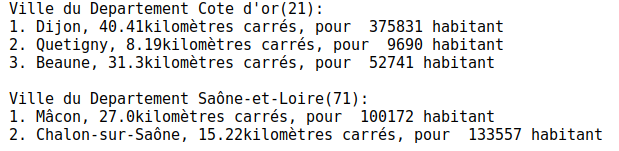
\includegraphics[width=400pt]{./tp/Pictures/tp1-execute}
  \caption{Éxécution TP1}
  \label{Éxécution TP1}
\end{figure}

\section{Exercice 4 : Attributs et méthodes de classe vs attributs et méthodes d'instances}
\textit{}
